\begin{figure}[htbp]
\centering
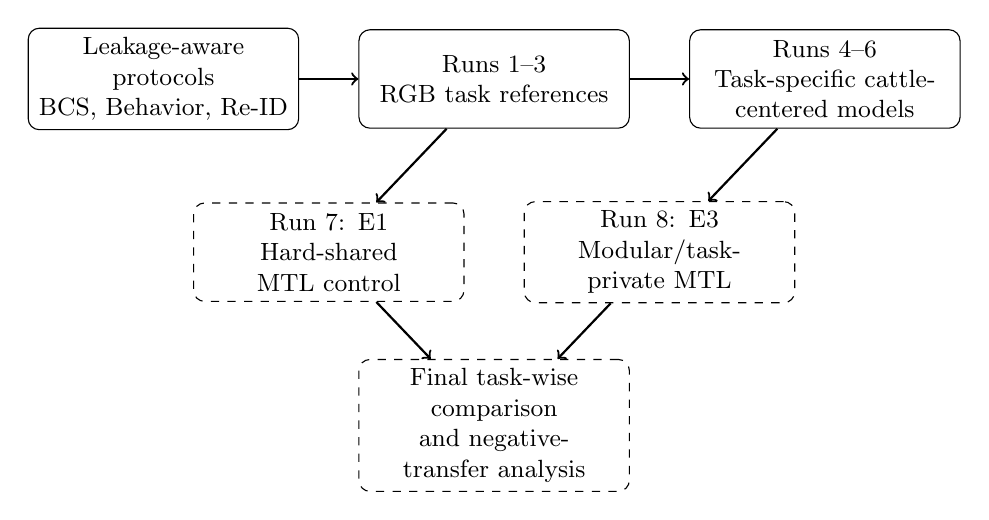
\begin{tikzpicture}[
  box/.style={draw,rounded corners,align=center,text width=3.2cm,minimum height=1.25cm,font=\small},
  pending/.style={box,dashed},
  arrow/.style={->,thick}
]
\node[box] (protocols) at (0,0) {Leakage-aware protocols\\BCS, Behavior, Re-ID};
\node[box] (rgb) at (4.2,0) {Runs 1--3\\RGB task references};
\node[box] (centered) at (8.4,0) {Runs 4--6\\Task-specific cattle-centered models};
\node[pending] (e1) at (2.1,-2.2) {Run 7: E1\\Hard-shared MTL control};
\node[pending] (e3) at (6.3,-2.2) {Run 8: E3\\Modular/task-private MTL};
\node[pending] (synthesis) at (4.2,-4.4) {Final task-wise comparison\\and negative-transfer analysis};
\draw[arrow] (protocols) -- (rgb);
\draw[arrow] (rgb) -- (centered);
\draw[arrow] (rgb) -- (e1);
\draw[arrow] (centered) -- (e3);
\draw[arrow] (e1) -- (synthesis);
\draw[arrow] (e3) -- (synthesis);
\end{tikzpicture}
\caption[Phase 3 comparative research design]{Phase 3 comparative design. Solid boxes are supported by completed Runs 1--6; dashed boxes identify the pending MTL experiments and final synthesis.}
\label{fig:phase3design}
\end{figure}
